\chapter{Methods}\label{ch:methods}
This chapter introduces the methods and theoretical background that is required to understand the Proximal Policy Optimization algorithm.
Section~\ref{sec:continuous-robotic-control} introduces the task of continuous robotic control, Section~\ref{sec:reinforcement-learning-basics}
provides an introduction to the basics of reinforcement learning, one of the fundamental papers for the PPO algorithm is discussed in Section~\ref{sec:trust-region-policy-optimization}.
Section~\ref{sec:proximal-policy-optimization} goes in depth on the PPO algorithm.


\section{Continuous Robotic Control}\label{sec:continuous-robotic-control}
Continuous robotic control in the context of reinforcement learning refers to the task of maximizing the reward of an agent
on a specific environment by providing a control signal to the robot that acts as the agent.
In many reinforcement learning tasks the state space and especially the action space are discrete.
For continuous robotic control commonly both the state space, and the action space are continuous as they model
the physical environment such as torques applied to actuators.
Due to the continuity of the action space, approaches such as Deep Q-Networks cannot be applied to continuous tasks
without modification as they suffer from the curse of dimensionality~\cite{Lillicrap2019}.
Thus, the need for more general algorithms that do not suffer from a high dimensional action space arises.
The problem formulation for the task of continuous robotic control is generally in the realm of control theory.
Especially optimal control theory is closely related to reinforcement learning~\cite{Gottschalk2019}.
Further, the considered tasks often contain very high dimensional state and action spaces.
An example is 3D robotic environments included in the openAI gym, e.g.\ the Humanoid-v2~\cite{brockman2016openai}.
For such high-dimensional problems especially with many actuators
the computation of a solution using optimal control theory may become time-consuming
as well as missing guarantees for the validity of the solution~\cite{Gottschalk2019}.
Thus, reinforcement learning based  solutions are of interest as their computational complexity
during inference mainly consists of the policy inference time without having to solve an optimization problem online.


\section{Reinforcement Learning Basics}\label{sec:reinforcement-learning-basics}
This section introduces the basic reinforcement learning framework.
In reinforcement learning the agent interacts with the environment by issuing actions and observing
the resulting state transition and reward~\cite{Sutton1998}.
This is visualized in Figure~\ref{fig:RL_env}.
\begin{figure}[t]
    \centering
    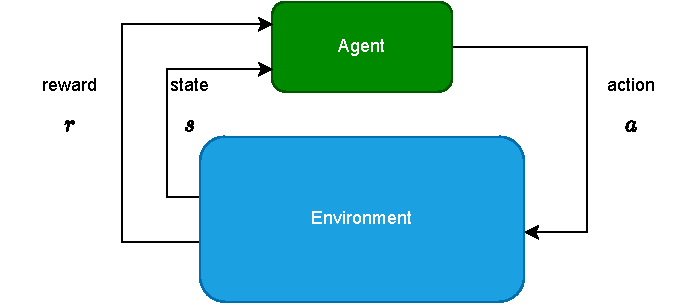
\includegraphics[width=0.5\textwidth]{images/presentation/RL_env.pdf}
    \caption{Interaction of the agent with the environment.}
    \label{fig:RL_env}
\end{figure}
Further, the environment is commonly described by a Markov Decision Process which is given by the tuple
$\{S, A, T, R, p(s_0), \gamma\}$ where $S$ is the set of states, $A$ the set of actions, $T: S\times A\to p(S)$ a transition
function, $R$ a reward function, $p(s_0)$ is the distribution for the initial state and
$\gamma$ is the discount factor~\cite{Moerland2020}.
Based on this, we define the policy as a function $\pi: S\times A \to p(S)$ and introduce the expected discounted reward~\cite{Schulman2015TrustRP}
\begin{equation}
    \eta(\pi) = \mathbb{E}\left[ \sum_{t=0}^\infty \gamma^t r(s_t) \right]
\end{equation}
where $s_0\sim p(s_0)$, $a_t\sim\pi(a_t|s_t)$ and $s_{t+1} \sim P(s_{t+1} | s_t, a_t)$.
Further, the state-action value function, value function and advantage function respectively are defined as
\begin{align}
    Q_\pi(s_t, a_t) &= \mathbb{E}\left[ \sum_{k=0}^\infty \gamma^kr(s_{t+k}) \right]\\
    V_{\pi}(s_t) &= \mathbb{E}\left[ \sum_{k=0}^\infty \gamma^k r(s_{t+k})  \right]\\
    A_{\pi}(s, a) &= Q_{\pi}(s,a) - V_{\pi}(s)
    \label{eq:advantage_fc}
\end{align}
where $a_t$ and $s_{t+1}$ are sampled from the respective distributions~\cite{Schulman2015TrustRP}.
There are many possible ways to learn in the above shown framework.
Trust Region Policy Optimization and Proximal Policy Optimization are both based on Policy Gradient methods.
Therefore, I will only discuss this in the following.
Now consider a policy $\pi_\theta$ which is parameterized by a set of parameters $\theta$.
The policy must be differentiable w.r.t.\ the parameters~\cite{Sutton1999}.
The basic premise of policy gradient methods is to compute an estimate of the policy gradient and perform gradient ascent
optimization based on the estimate.
One such estimator is given by
\begin{equation}
    \Hat{g} = \mathbb{E}\left[ \nabla_\theta \log(\pi_\theta(a_t | s_t)) \Hat{A}_t\right]
\end{equation}
where $\nabla_\theta$ denotes the gradient w.r.t. the parameters and $\Hat{A}_t$ the estimate of the advantage function~\cite{schulman2017ppo}.

\section{Trust Region Policy Optimization}\label{sec:trust-region-policy-optimization}
Trust Region Policy Optimization plays a vital role in understanding the Proximal Policy Optimization algorithm.
Based on the framework introduced in Section~\ref{sec:reinforcement-learning-basics} a monotonic improvement guarantee can be formulated.
One of the main contributions is the proof that such a monotonic improvement guarantee can be obtained not just for mixture policies but
also general stochastic policies which includes neural networks~\cite{Schulman2015TrustRP}.
This leads to the following theorem~\cite{Schulman2015TrustRP}:
Let
\begin{equation}
    \alpha=\max_s\left \{ \frac{1}{2} \sum_i |\pi(\cdot|s)_i - \Tilde{\pi}(\cdot|s)_i| \right\}
\end{equation}
be the total variation divergence between
the old and the new policy.
Then the following bound holds
\begin{equation}
    \eta(\Tilde{\pi}) \geq L_{\pi}(\Tilde{\pi}) - \frac{4\varepsilon\gamma}{(1-\gamma)^2}\alpha^2
\end{equation}
where $\pi$ is the old policy, $\Tilde{\pi}$ the new policy, $\gamma$ the discount factor,
$\varepsilon = \max_{s,a} \left\{ |A_\pi(s,a)| \right\}$ and $L(\cdot)$ is a local approximation of the
discounted reward $\eta$ given by
\begin{equation}
    L_{\pi}(\Tilde{\pi}) = \eta(\pi) + \sum_s p_{\pi}(s) \sum_a \Tilde{\pi}(a|s) A_{\pi}(s, a)
\end{equation}
The same can be formulated using the Kullback-Leibler divergence instead of the total variation divergence which results in
\begin{equation}
    \eta(\Tilde{\pi}) \geq L_{\pi}(\Tilde{\pi}) - C D_{KL}^{max}(\pi, \Tilde{\pi})
\end{equation}
where $C = \frac{4\varepsilon\gamma}{(1-\gamma)^2}$~\cite{Schulman2015TrustRP}.
This allows for a chain of monotonically improving policies $\pi$.
To obtain a practical algorithm two further problems must be solved.
The policy cannot be evaluated at every state $s$ which is why the optimization problem is posed as follows
\begin{equation}
    \max_{\Tilde{\theta}} L_{\pi_{\theta}}(\pi_{\Tilde{\theta}})
\end{equation}
subject to $\mathbb{E}\left[ D_{KL}(\pi_\theta || \pi_{\Tilde{\theta}}) \right] \leq \delta$.
Here $\delta$ controls the maximum update step size of the policy.
Lastly, the formulation of the optimization problem must be converted to sample-based estimation of the
objective function and the constraint.
A practical formulation of the Trust Region Policy Optimization algorithm is shown in Algorithm~\ref{alg:trpo}.
\begin{algorithm}
\caption{Trust Region Policy Optimization - Practical Algorithm}
    \begin{algorithmic}
        \Require  Hyperparameter $N, T, \dots$

        \While{termination criterion not met}
        \For{actor=$1,\dots,N$}
            \State Collect rollout buffer for $T$ steps
            \State Compute Monte-Carlo estimates of Q-values
        \EndFor
        \State Compute sample-based expectations of the objective and constraint
        \State Solve constrained optimization (conjugate gradients and line search)
        \EndWhile
    \end{algorithmic}
    \label{alg:trpo}
\end{algorithm}
Note that the conjugate gradients procedure requires second derivatives which are computationally expensive to obtain.

\section{Proximal Policy Optimization}\label{sec:proximal-policy-optimization}
The fundamental goal of the Proximal Policy Algorithm is to preserve the advantages of TRPO while using simple first-order
optimization methods which results in a simple and more efficient implementation~\cite{schulman2017ppo}.
PPO builds on the previously introduced policy gradient methods and TRPO by introducing the concept of a surrogate function
which is optimized instead.
The surrogate objective I used in the implementation and that achieved the best results is the clipped surrogate objective
which is given by
\begin{equation}
    L_{CPI}(\theta) = \Hat{\mathbb{E}}_t \left[ \frac{\pi_\theta(a_t | s_t)}{\pi_{\theta_{old}}(a_t | s_t)}\cdot \Hat{A}_t \right] = \Hat{\mathbb{E}}\left[ r_t(\theta)\Hat{A}_t \right]
\end{equation}
where $\Hat{A}_t$ is the advantage function estimate.
However, this does not account for the limited update of the policy introduced in TRPO.
Thus, excessively large policy updates are expected~\cite{schulman2017ppo}.
The clipped function is given by
\begin{equation}
    L_{CLIP}(\theta) = \Hat{\mathbb{E}}\left[ \min\left\{ r_t(\theta)\Hat{A}_t, \operatorname{clip}(r_t(\theta), 1-\varepsilon, 1+\varepsilon) \Hat{A}_t \right\} \right]
\end{equation}
where $\varepsilon$ is a hyperparameter controlling the largest possible policy update.
A common trick during implementation is to normalize the advantage function estimate to zero-mean and unit-variance to
increase stability during training.
A second proposed surrogate function is the adaptive KL penalty coefficient surrogate function which is given by
\begin{equation}
    L_{KLPEN}(\theta) = \Hat{\mathbb{E}}\left[ \frac{\pi_\theta(a_t | s_t)}{\pi_{\theta_{old}}(a_t | s_t)}\cdot \Hat{A}_t - \beta D_{KL}(\pi_{\theta_{old}} || \pi_\theta) \right]
\end{equation}
where the penalty coefficient $\beta$ is either halfed or doubled based on a target KL-Divergence hyperparameter~\cite{schulman2017ppo}.
The Proximal Policy Algorithm in the Actor-Critic implementation is shown in Algorithm~\ref{alg:ppo}~\cite{schulman2017ppo}.
\begin{algorithm}
\caption{Proximal Policy Optimization - Actor-Critic Implementation}\label{alg:ppo}
    \begin{algorithmic}
        \Require  Hyperparameter $\varepsilon, N, T, K, \dots$
        \While{termination criterion not met}
        \For{actor=$1,\dots,N$}
            \State Collect rollout buffer using current policy $\pi_{\theta_{old}}$ for $T$ steps
            \State Compute advantage function estimate $\Hat{A}_1, \dots, \Hat{A}_T$
        \EndFor
        \For{epoch=$1,\dots,K$}
            \State Optimize surrogate function $L$ w.r.t. $\theta$
            \State Update policy $\theta_{old} \leftarrow \theta$
        \EndFor
        \EndWhile
    \end{algorithmic}
\end{algorithm}
The training loop is repeated until the termination criterion is met which is given by a total number of training steps.
In a first step a rollout buffer is collected which contains a list of the visited states, the actions and observed rewards.
Based on the collected rollout buffer the advantage function estimate is computed.
For this, the value function is evaluated,  and the advantage function is computed following Equation~\ref{eq:advantage_fc}.
In particular, the rewards-to-go are required for the estimation.
The rewards-to-go or discounted rewards are computed for each episode in the rollout buffer by iterating the rewards
in reverse order and adding the current reward to the discounted sum.
The value function and policy are both given by neural networks which are optimized for $K$ epochs.
The policy network uses the surrogate objective function for gradient ascent.
Further, a Huber loss is employed for the optimization of the value function network.
The PPO algorithm is very flexible to different implementations regarding the modeling of the policy and value function.
For simplicity, I have decided to model both as separate neural networks but parameter sharing between the networks is possible.
This influences the computation of the surrogate / loss function.
The architecture of the policy network is shown in Figure~\ref{fig:policy_mlp}.
A simple Multi-Layer Perceptron network with three layers is used, each layer using a $\operatorname{Tanh}(\cdot)$ activation~\cite{Goodfellow-et-al-2016}.
The output of the policy network is a mean-value which is used to construct a multi-variate gaussian distribution from which an action is sampled.
Note that the covariance is initialized as a diagonal matrix as it is assumed that there exist no dependencies between
the components.
In the following the variance used to initialize the covariance matrix is referred to as $\sigma$.
The architecture is shared by the value function network without the action sampling.
\begin{figure}[t]
    \centering
    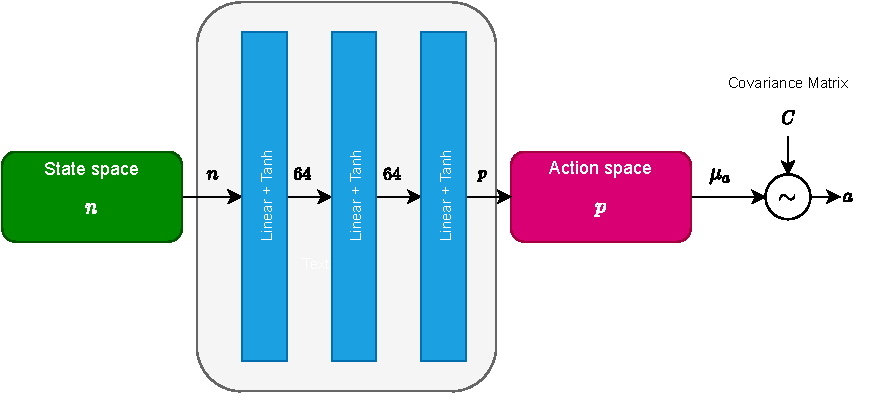
\includegraphics[width=0.7\textwidth]{images/presentation/ann_policy_value.pdf}
    \caption{Architecture of the policy MLP.}
    \label{fig:policy_mlp}
\end{figure}
